\documentclass[11pt]{jarticle}

\usepackage[dvipdfmx]{graphicx}
\usepackage{listings}

\lstset{
    basicstyle={\ttfamily\small}, %書体の指定
    frame=tRBl, %フレームの指定
    framesep=10pt, %フレームと中身(コード)の間隔
    breaklines=true, %行が長くなった場合の改行
    linewidth=12cm, %フレームの横幅
    lineskip=-0.5ex, %行間の調整
    tabsize=2 %Tabを何文字幅にするかの指定
}

\setlength{\oddsidemargin}{-6.35mm}
\setlength{\textwidth}{171.9mm}

\begin{document}

\title{画像処理実験 第2回}
\author{09430565\\大橋虎ノ介}
\date{\number\year 年\number\month 月\number\day 日}
\maketitle

\section{[2.1]}
(x,y)と(u,v)の位置に,ほぼ同じ物体が観測されていることを確認した.

\section{画像の幾何学変換}

\[
  a = \left(
    \begin{array}{ccc}
      1 & 0 & 0 \\
      0 & 1 & 0 \\
      0 & 0 & 1
    \end{array}
  \right)
\]

としたとき以下のような画像が得られた

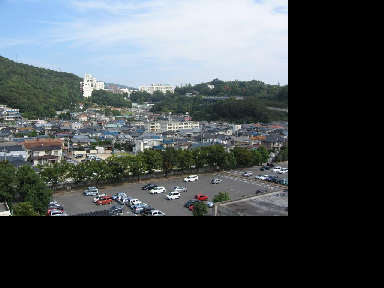
\includegraphics[scale=.5]{./img/download.png}

また,C言語で同様の処理を行った結果,以下の画像が得られた.

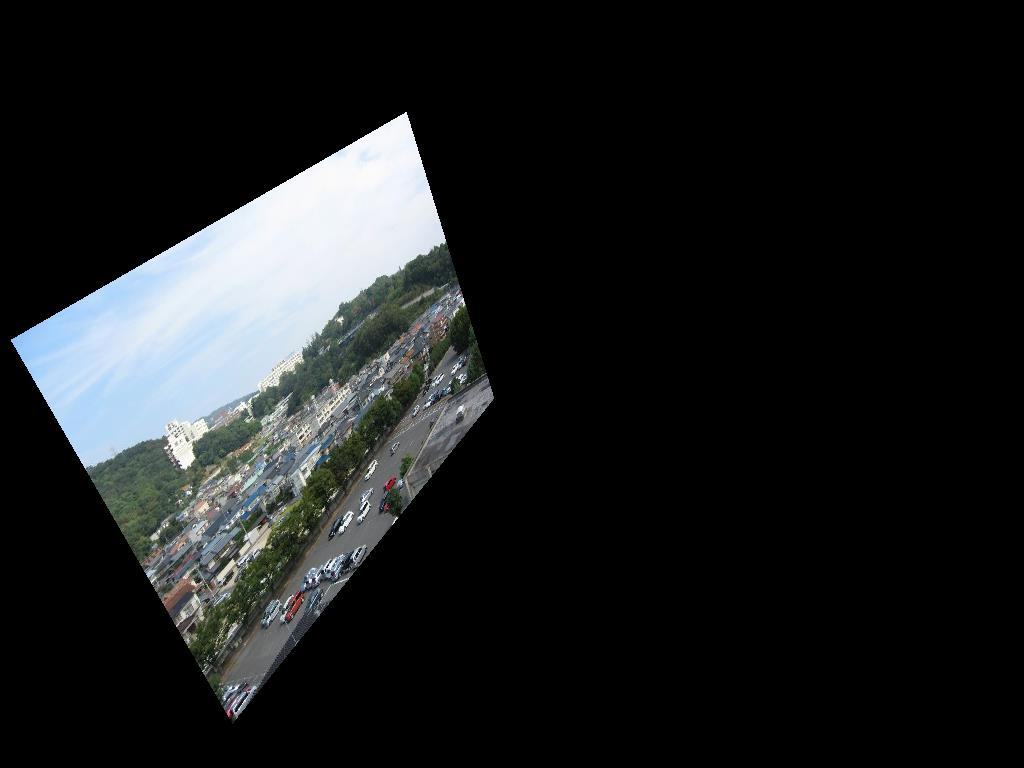
\includegraphics[scale=.5]{./img/c_henkan.jpg}

\section{[2.2]}

\[
  m0d = \left(
    \begin{array}{ccc}
      2 & 0 & -100 \\
      0 & 2.667 & -100 \\
      0 & 0 & 0.5
    \end{array}
  \right)
\]
に変更してもimg1とimg2の位置関係が保たれることを確認した.

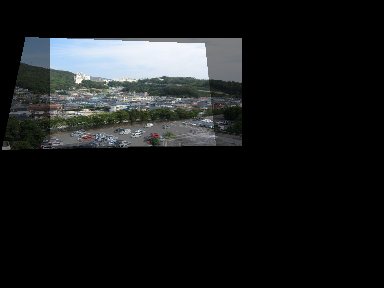
\includegraphics[scale=.5]{./img/img01.png}


\[
  m10 = \left(
    \begin{array}{ccc}
        0.915825 & 0.027095 & 122.163930 \\
        -0.057781 & 1.013717 & 18.545453 \\
        -0.000156 & 0.000078 & 1.000000
    \end{array}
  \right)
\] 
ずれのない画像を作成した.

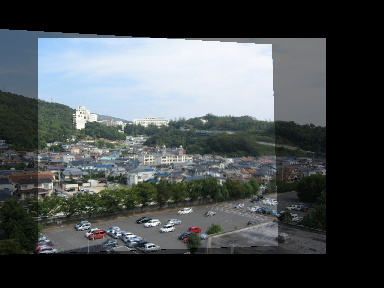
\includegraphics[scale=.5]{./img/zurenashi.png}

\section{[2.3]}

3x3 行列の積を計算する関数 mult33 を以下のように実装し,画像を合成した.

\begin{lstlisting}
    
void mult33(double d[3][3], double a[3][3], double b[3][3]) {
	int x, y, i;

	for (y = 0; y < 3; y++)
		for (x = 0; x < 3; x++) {
			d[y][x] = 0;
			for (i = 0; i < 3; i++){
				d[y][x] += a[y][i] * b[i][x];
			}
		}
}
\end{lstlisting}

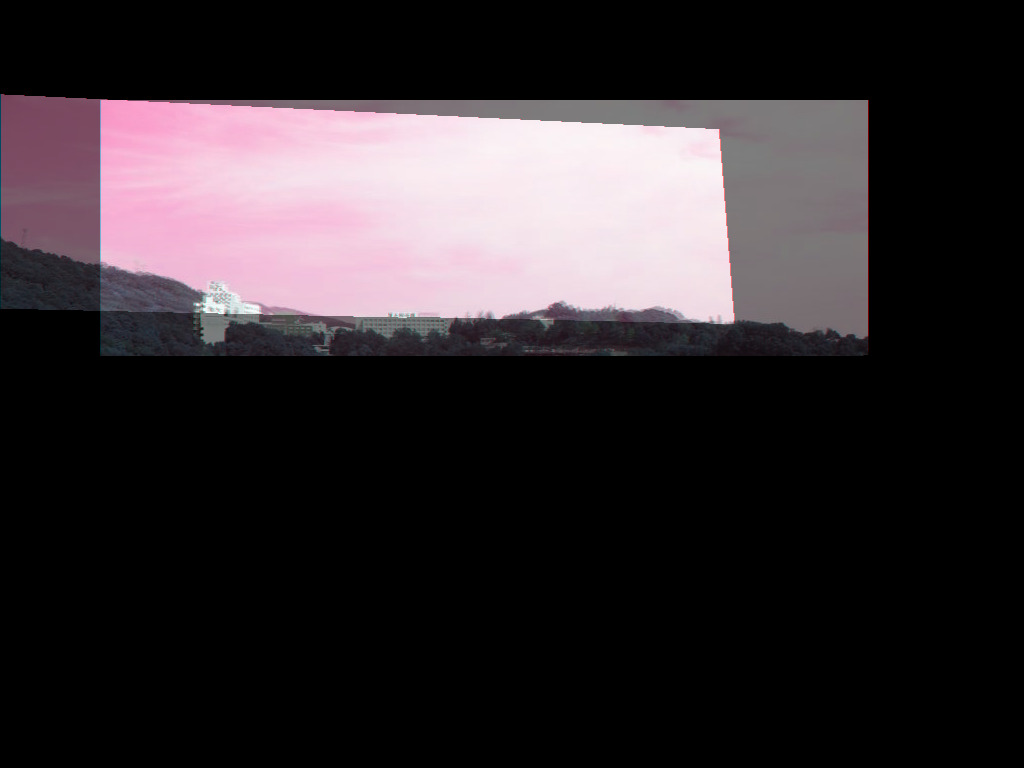
\includegraphics[scale=.5]{./img/out.jpg}

画像の色がおかしく,一部がかけている.

\section{[2.4]考察と感想}
「原画像の座標(u,v)を出力画像の座標(x,y)に変換する行列」を A とする.
式で表すと以下になる.
\[
    \left(
        \begin{array}{c}
           x \\
           y 
        \end{array}
      \right)
      =A
    \left(
    \begin{array}{c}
       u \\
       v 
    \end{array}
  \right)
\]

上記の実装では,出力画像の座標に対応する現画像の座標を求めていた.

\[
    \left(
        \begin{array}{c}
           u \\
           v 
        \end{array}
      \right)
      =a
    \left(
    \begin{array}{c}
       x \\
       y 
    \end{array}
  \right)
\]

このaは上式のAの逆行列に等しい.

\[
    \left(
        \begin{array}{c}
           u \\
           v 
        \end{array}
      \right)
      =A^{-1}
    \left(
    \begin{array}{c}
       x \\
       y 
    \end{array}
  \right)
\]


[2.3]で行ったc言語での実装では,画像の欠けと色がおかしいことを確認した.
プログラムを実行した際に

\begin{lstlisting}
    convert: unable to write file `-' @ error/constitute.c/WriteImage/1283.
\end{lstlisting}
という警告かエラーをはいたのでそれが原因ではないかと思う.

\end{document}
